\documentclass[12pt, a4paper]{report}

% ─── Typography & Page Geometry ───────────────────────────────────────────────
\usepackage[a4paper, top=1in, bottom=1in, left=1.25in, right=1in]{geometry}
\usepackage{setspace}
\setstretch{1.25}

\usepackage{fontspec}
\defaultfontfeatures{Ligatures=TeX}
\setmainfont{Times New Roman}
\setmonofont{Consolas}[Scale=0.92]
\newfontfamily\bengalifont{Kalpurush}[Script=Bengali,AutoFakeBold=1.5]

% Automatic font switching for Bengali Unicode range
\usepackage{ucharclasses}
\setTransitionsFor{Bengali}{\bengalifont}{\rmfamily}

\setlength{\parskip}{5pt plus 1pt minus 1pt}
\setlength{\parindent}{0pt}

% ─── Standard Packages ────────────────────────────────────────────────────────
\usepackage{amsmath,amssymb}
\usepackage{graphicx}
\usepackage{xcolor}
\usepackage{booktabs}
\usepackage{longtable}
\usepackage{tabularx}
\usepackage{array}
\usepackage{multicol}
\graphicspath{{./}{./img/}{./diagrams/}}
\usepackage{fancyhdr}
\usepackage{titlesec}
\usepackage[font={small,rm},labelfont={bf,rm},labelsep=period]{caption}
\usepackage{listings}
\usepackage{tcolorbox}
\tcbuselibrary{skins,breakable}
\usepackage{tikz}
\usetikzlibrary{shapes.geometric, arrows.meta, positioning, calc, fit}
\usepackage{float}
\usepackage{microtype}
\setlength{\emergencystretch}{3em}

% ─── Professional Academic Headings (Times New Roman) ─────────────────────────
\titleformat{\chapter}[display]
  {\normalfont\bfseries}
  {\large\MakeUppercase{\chaptertitlename}\ \thechapter}
  {6pt}
  {\LARGE\bfseries}
\titlespacing*{\chapter}{0pt}{-10pt}{18pt}

\titleformat{\section}
  {\normalfont\Large\bfseries}
  {\thesection}{1em}{}
\titlespacing*{\section}{0pt}{12pt}{5pt}

\titleformat{\subsection}
  {\normalfont\large\bfseries}
  {\thesubsection}{1em}{}
\titlespacing*{\subsection}{0pt}{10pt}{4pt}

\titleformat{\subsubsection}
  {\normalfont\normalsize\bfseries}
  {\thesubsubsection}{1em}{}
\titlespacing*{\subsubsection}{0pt}{8pt}{3pt}

% ─── Dedicated UML Space Macro ───────────────────────────────────────────────
\newcommand{\umlspacesection}[4]{%
\begin{figure}[H]
\centering
\vspace{-0.2cm}
\IfFileExists{#3}{%
    \centerline{\includegraphics[#4]{#3}}%
}{%
    \begin{tcolorbox}[
        enhanced,
        width=0.98\textwidth,
        height=12cm,
        colback=gray!3,
        colframe=blue!75!black,
        boxrule=1.2pt,
        arc=4pt,
        halign=center,
        valign=center,
        title=\textbf{#2}
    ]
        \vspace*{\fill}
        {\Large\bfseries [ Space Reserved for UML Diagram ]}\par\vspace{0.35cm}
        {\large\bfseries #2}\par\vspace{0.25cm}
        {\small\color{black!75}\textbf{Target Graphic File:} \texttt{\detokenize{#3}}}\par\vspace{0.2cm}
        {\footnotesize\color{black!60} (Dedicated reserved space for diagram image / print attachment. Interactive source: \texttt{diagrams/view\_uml.html})}\par
        \vspace*{\fill}
    \end{tcolorbox}
}
\vspace{-0.1cm}
\caption{#2}
\label{#1}
\end{figure}
}

\usepackage{hyperref}
\hypersetup{
    colorlinks=true,
    linkcolor=black,
    citecolor=black,
    urlcolor=blue!75!black,
    linktoc=all,
    bookmarks=true,
    bookmarksnumbered=true,
    bookmarksopen=true,
    pdfborder={0 0 0},
    pdftitle={BornoCompiler: A Native Bangla Programming Language Compiler},
    pdfauthor={Mumshad Chowdhury Mahdi, Sharon Shahrin Mim, Tasmina Rahman Chowdhury}
}

% ─── Header & Footer Settings ────────────────────────────────────────────────
\setlength{\headheight}{15pt}
\addtolength{\topmargin}{-3pt}
\pagestyle{fancy}
\fancyhf{}
\fancyhead[L]{\small\rmfamily\slshape BornoCompiler: Final Project Report}
\fancyhead[R]{\small\rmfamily\slshape\nouppercase{\leftmark}}
\fancyfoot[C]{\rmfamily\thepage}
\renewcommand{\headrulewidth}{0.5pt}

\fancypagestyle{plain}{
    \fancyhf{}
    \fancyfoot[C]{\rmfamily\thepage}
    \renewcommand{\headrulewidth}{0pt}
}

% ─── Code Listing Configuration ──────────────────────────────────────────────
\definecolor{codegray}{gray}{0.96}
\definecolor{codelinegray}{gray}{0.4}
\definecolor{keywordblue}{RGB}{20, 50, 160}

\lstset{
    basicstyle=\ttfamily\small,
    backgroundcolor=\color{codegray},
    frame=single,
    rulecolor=\color{black!20},
    breaklines=true,
    breakatwhitespace=false,
    columns=fullflexible,
    keepspaces=true,
    showstringspaces=false,
    tabsize=4,
    xleftmargin=12pt,
    xrightmargin=12pt,
    framesep=6pt
}

% ─── Document Body ───────────────────────────────────────────────────────────
\begin{document}

% ─── Cover & Preliminary Formal Pages (Leading University Template) ──────────
\begin{titlepage}
\thispagestyle{empty}

\begin{center}
    {\huge\bfseries Leading University}\\[0.25cm]
    {\LARGE\bfseries Department of Computer Science and Engineering}\\[0.4cm]
    {\LARGE\bfseries Course Code: CSE 4114}
    
    \vfill
    
\includegraphics[width=3.2cm,keepaspectratio]{./img/LU}
    \vfill
    
    {\LARGE\bfseries BornoCompiler: A Native Bangla Programming Language Compiler}\\[0.6cm]
    
    {\large\bfseries Team: Symbol Table}\\[0.4cm]
    
    \begin{multicols}{2}
        \textbf{Mumshad Chowdhury Mahdi}\\
        \textbf{Sharon Shahrin Mim}\\
        \textbf{Tasmina Rahman Chowdhury}\\[0.2cm]
        \columnbreak
        ID: 0182320012101083\\
        ID: 0182320012101064\\
        ID: 0182320012101050
    \end{multicols}
    
    \vspace{0.4cm}
    Department of Computer Science and Engineering\\
    Leading University, Sylhet, Bangladesh
    
    \vfill
    {\bfseries Supervisor}\\[0.15cm]
    \textbf{Alian Ahmed Ferdous}\\
    Adjunct Lecturer\\ 
    Department of Computer Science and Engineering\\
    Leading University, Sylhet, Bangladesh
    
    \vfill
    \today
    
    % ─── Page 2: Inner Submission Page ───────────────────────────────────────
    \newpage
    \thispagestyle{empty}
    {\Large\bfseries BornoCompiler: A Native Bangla Programming Language Compiler}\\[0.4cm]
    
    \vspace{0.2cm}
    
\includegraphics[width=3.2cm,keepaspectratio]{./img/LU}\\[0.4cm]
    
    A Project\\
    submitted to the\\[0.2cm]
    {\large Department of Computer Science and Engineering}\\[0.2cm]
    {\Large Leading University}\\
    Sylhet - 3112, Bangladesh\\[0.5cm]
    
    in partial fulfillment of the\\
    requirements for the degree of\\[0.3cm]
    {\Large Bachelor of Science in Computer Science and Engineering}
    
    \vfill
    {\LARGE By}\\[0.2cm]
    {\large\bfseries Team: Symbol Table}\\[0.4cm]
    
    \begin{multicols}{2}
        \textbf{Mumshad Chowdhury Mahdi}\\
        \textbf{Sharon Shahrin Mim}\\
        \textbf{Tasmina Rahman Chowdhury}\\[0.2cm]
        \columnbreak
        ID: 0182320012101083\\
        ID: 0182320012101064\\
        ID: 0182320012101050
    \end{multicols}
    
    \vfill
    {\bfseries Supervisor}\\[0.15cm]
    \textbf{Alian Ahmed Ferdous}\\
    Adjunct Lecturer\\ 
    Department of Computer Science and Engineering\\
    Leading University, Sylhet, Bangladesh
    
    \vfill
    \today
    
\end{center}

% ─── Page 3: Recommendation Letter from Project Supervisor ───────────────────
\newpage
\thispagestyle{empty}
\begin{center}
    \textbf{\huge Recommendation Letter from the Project Supervisor}
\end{center}
\vspace{0.8cm}

\noindent
The project entitled ``\emph{BornoCompiler: A Native Bangla Programming Language Compiler}'' submitted by the students of \textbf{Team: Symbol Table}:
\begin{enumerate}
    \item \textbf{Mumshad Chowdhury Mahdi}, ID: 0182320012101083
    \item \textbf{Sharon Shahrin Mim}, ID: 0182320012101064
    \item \textbf{Tasmina Rahman Chowdhury}, ID: 0182320012101050
\end{enumerate}
\vspace{0.3cm}
\noindent
This is a record of research work carried out under my supervision, and I hereby approve that the report be submitted in partial fulfillment of the requirements for the award of their bachelor's degrees.

\vspace{7.5cm}
\noindent
Signature of the Supervisor: \\[0.3cm]
\textbf{Alian Ahmed Ferdous}\\
Adjunct Lecturer\\
Department of Computer Science and Engineering\\
Leading University, Sylhet\\[0.15cm]
Date: \today

% ─── Page 4: Certificate of Acceptance of the Project ────────────────────────
\newpage
\thispagestyle{empty}
\begin{center}
    \textbf{\huge Certificate of Acceptance of the Project}
\end{center}
\vspace{0.8cm}

\noindent
The project entitled ``\emph{BornoCompiler: A Native Bangla Programming Language Compiler}''\\
submitted by the students of \textbf{Team: Symbol Table}:
\begin{enumerate}
    \item \textbf{Mumshad Chowdhury Mahdi}, ID: 0182320012101083
    \item \textbf{Sharon Shahrin Mim}, ID: 0182320012101064
    \item \textbf{Tasmina Rahman Chowdhury}, ID: 0182320012101050
\end{enumerate}
on \today

\vspace{0.3cm}
\noindent
is hereby accepted in partial fulfillment of the requirements for the award of the degree of Bachelor of Science in Computer Science and Engineering.

\vspace{5.2cm}

\begin{multicols}{3}
    \begin{flushleft}
        \hrulefill \\
        {\footnotesize \textbf{Chairman, Defence Board}\\\vspace{1mm}Name:\\
        Designation:\\Department of CSE}
    \end{flushleft}

    \begin{flushleft}
        \hrulefill \\
        {\footnotesize \textbf{Member 1, Defence Board}\\\vspace{1mm}Name:\\
        Designation:\\Department of CSE}
    \end{flushleft}

    \begin{flushleft}
        \hrulefill \\
        {\footnotesize \textbf{Member 2, Defence Board}\\\vspace{1mm}Name:\\
        Designation:\\Department of CSE}
    \end{flushleft}
\end{multicols}

\end{titlepage}

% ─── Abstract ────────────────────────────────────────────────────────────────
\pagenumbering{roman}
\setcounter{page}{1}

\begin{abstract}
\noindent This report presents the architectural specification, formal grammar, semantic validation framework, and multi-target code generation engine of \textbf{BornoCompiler}, an academic compiler designed and constructed from scratch for \textbf{Borno}—an imperative, statically typed programming language written using the native script and lexicon of the Bangla language (বাংলা). Built entirely in Java without external parser-generator dependencies, BornoCompiler implements an end-to-end six-phase pipeline: character-level Unicode lexical analysis with source-coordinate tracking, recursive-descent LL(1) parsing with panic-mode error recovery, strongly typed Abstract Syntax Tree (AST) synthesis, lexically scoped semantic analysis with static compile-time division-by-zero detection, intermediate representation via linearized Three Address Code (TAC), and dual target code generation emitting clean, indented Python 3 source code as well as low-level WebAssembly Text Format (\texttt{.wat}). The compiler is validated against a comprehensive test suite of 28 structured test cases and a dedicated regression test harness covering complex operator precedence, nested conditional branching, and iterative loops (\texttt{যতক্ষণ}, \texttt{ফর}). This report documents the exact implementation, class hierarchies, intermediate representation quadruples, and grammar productions as realized in the project codebase.
\end{abstract}

\tableofcontents
\listoffigures
\listoftables

\clearpage
\pagenumbering{arabic}
\setcounter{page}{1}

% ─── Chapter 1: The Pitch ────────────────────────────────────────────────────
\chapter{The Pitch}

\section{Introduction}
Computing and programming education are predominantly framed through the lens of Latin-derived languages. Mainstream languages—ranging from C, C++, and Java to Python and JavaScript—mandate English keywords (\texttt{let}, \texttt{int}, \texttt{if}, \texttt{while}, \texttt{print}), ASCII-based punctuation, and English standard library functions. For millions of non-English native speakers, learning computational problem-solving entails confronting two formidable intellectual hurdles simultaneously: understanding abstract algorithmic logic and navigating foreign linguistic syntax.

\textbf{BornoCompiler} is an authentic, university-standard compiler engineered from the ground up in Java to compile \textbf{Borno}, a programming language structured completely around the phonetic rules, vocabulary, and Unicode script of the Bangla language. Unlike superficial preprocessing scripts that simply replace keywords before piping text into an off-the-shelf runtime, BornoCompiler establishes an independent, complete compilation pipeline. It tokenizes raw Unicode text, parses syntax according to a formal context-free grammar, validates semantic consistency across lexical scopes, transforms programs into an intermediate Three Address Code (TAC) representation, and synthesizes target outputs for both high-level scripting environments (Python 3) and web/system virtual machines (WebAssembly).

\section{Motivation}
With over 300 million native speakers worldwide, Bangla is the fifth most spoken native language globally. Within Bangladesh and the state of West Bengal, India, students encountering computer science at the primary, secondary, and introductory undergraduate levels frequently experience cognitive friction when deciphering English keywords.

When a student writes:
\begin{center}
\texttt{ধরি সংখ্যা বয়স = ২০;}
\end{center}
the conceptual alignment between natural cognition and code syntax is immediate. The student understands \texttt{ধরি} as variable initialization, \texttt{সংখ্যা} as numeric type binding, \texttt{বয়স} as the identifier, and \texttt{২০} as the literal. The cognitive overhead of linguistic translation is eliminated, allowing instructional focus to center entirely on data structures, algorithmic flow, operator precedence, and memory mutation.

\section{Problem Statement}
Prior initiatives attempting to introduce non-English educational programming typically suffer from two severe technical flaws:
\begin{enumerate}
    \item \textbf{Text-Substitution Wrapper Flaw}: Many existing systems are naive preprocessors that perform basic regex substitutions, mapping Bangla words to English tokens before calling an external Python or C interpreter. These tools cannot provide accurate syntax error diagnostics with line/column coordinates in the native language, nor do they teach students how compilers actually analyze and lower high-level constructs.
    \item \textbf{Absence of Intermediate Representation and Real Targets}: Educational toy compilers often evaluate an Abstract Syntax Tree directly via tree-walking interpreters, bypassing Intermediate Representation (IR) generation, control-flow linearization, and machine-level compilation targets.
\end{enumerate}
BornoCompiler solves this challenge by implementing a complete compiler architecture from scratch, producing Three Address Code, Python 3, and WebAssembly Text Format directly from source code.

\section{Objectives}
The core technical objectives accomplished in BornoCompiler are:
\begin{itemize}
    \item \textbf{Native Unicode Lexical Analysis}: Construct a deterministic scanner that recognizes pure Bangla Unicode code points (\texttt{\textbackslash u0980}--\texttt{\textbackslash u09FF}), handles Zero-Width Non-Joiner (ZWNJ) and Zero-Width Joiner (ZWJ) characters, tokenizes native Bangla digits (\texttt{০}--\texttt{৯}), and strictly enforces language purity by rejecting unauthorized Latin characters.
    \item \textbf{Resilient LL(1) Parsing}: Implement a recursive-descent parser equipped with panic-mode error recovery (\texttt{synchronize()}) that avoids cascading crashes and isolates syntax faults.
    \item \textbf{Object-Oriented AST Construction}: Produce an explicit, typed Abstract Syntax Tree capturing program semantics independently of lexical tokens.
    \item \textbf{Scoped Semantic Analysis}: Enforce lexical scope hierarchies with parent links, verify variable declarations and type compatibility, and evaluate expressions at compile time to catch semantic bugs like division by zero.
    \item \textbf{Intermediate Code Generation (TAC)}: Flatten complex expressions and control flow into Three Address Code instructions using sequential temporaries (\texttt{t1}, \texttt{t2}, \dots) and branch labels (\texttt{L1}, \texttt{L2}, \dots).
    \item \textbf{Multi-Target Code Emission}: Synthesize executable Python 3 code and standard WebAssembly Text Format (\texttt{.wat}) capable of direct execution in web browsers and standalone WASM runtimes.
\end{itemize}

\section{Real-World Use Cases}
\begin{itemize}
    \item \textbf{Introductory Computing in Schools}: Allowing primary and secondary schools across Bangladesh to introduce computational thinking and basic programming without requiring prior English fluency.
    \item \textbf{Undergraduate Compiler Pedagogy}: Serving as an open, readable, and formally structured codebase for university courses covering compiler design, parsing algorithms, scoped symbol tables, and bytecode/WASM generation.
    \item \textbf{Vocational Training Centers}: Providing vocational institutes in rural regions with an intuitive medium to train students in fundamental logical programming.
\end{itemize}

\section{Target Users}
\begin{itemize}
    \item \textbf{Bangla-Speaking Beginners}: Novices seeking to grasp core programming constructs (variables, branching, loops) without language barriers.
    \item \textbf{Computer Science Students}: Undergraduates learning how compilers parse, analyze, optimize, and translate code.
    \item \textbf{Academic Instructors}: Educators who require a clean, native reference implementation for classroom instruction.
\end{itemize}

\section{Long-Term Vision}
\textit{While the current implementation fulfills all course and compiler requirements, the long-term vision for Borno envisions:}\\
Developing a dedicated graphical IDE with real-time Bangla syntax highlighting; extending grammar support to user-defined functions, procedures, parameter passing, and arrays; and implementing direct native machine-code emission via LLVM.

% ─── Chapter 2: Language Overview ────────────────────────────────────────────
\chapter{Language Overview}

\section{Introduction to Borno}
\textbf{Borno} (বর্ণ, meaning \textit{character} or \textit{letter}) is a statically typed, imperative programming language. Statements terminate explicitly with a semicolon (\texttt{;}), code blocks are demarcated by curly braces (\texttt{\{ \}}), and expressions adhere to standard mathematical operator precedence.

\section{Design Goals}
\begin{itemize}
    \item \textbf{Syntactic Rigor}: Borno avoids loose, dynamic typing. Every variable has a declared type, conditions must evaluate strictly to boolean values, and undeclared identifiers are rejected at compile time.
    \item \textbf{Linguistic Authenticity}: Keywords represent natural, mathematically accepted Bangla words (\texttt{ধরি}, \texttt{সংখ্যা}, \texttt{বাক্য}, \texttt{যদি}, \texttt{নাহলে}, \texttt{যতক্ষণ}, \texttt{ফর}, \texttt{দেখাও}).
    \item \textbf{Pinpoint Diagnostic Feedback}: The compiler tracks source lines and columns, reporting detailed error messages directly in Bangla.
\end{itemize}

\section{Supported Data Types}
Borno implements three concrete primitive types managed through \texttt{Type.java}:
\begin{table}[htbp]
\centering
\small
\renewcommand{\arraystretch}{1.25}
\begin{tabular}{|l|l|l|l|}
\hline
\textbf{Borno Keyword} & \textbf{Internal Type} & \textbf{Semantic Description} & \textbf{Example Literals} \\
\hline
\texttt{সংখ্যা} & \texttt{NUMBER} & Double-precision float / integer & \texttt{০}, \texttt{১০}, \texttt{২০}, \texttt{৩.১৪১৬} \\
\hline
\texttt{বাক্য} / \texttt{লেখা} & \texttt{STRING} & UTF-8 double-quoted string & \texttt{"মাহদি"}, \texttt{"বাংলাদেশ"} \\
\hline
\textit{(Inferred)} & \texttt{BOOLEAN} & Truth value produced by comparisons & \texttt{ক > ৫}, \texttt{বয়স >= ১৮} \\
\hline
\end{tabular}
\caption{Supported Data Types in Borno}
\label{tab:data_types}
\end{table}

\section{Variables and Declarations}
Variable declarations begin with the optional keyword \texttt{ধরি} (let/assume), followed by the type specifier (\texttt{সংখ্যা} or \texttt{বাক্য}), an identifier in Bangla script, an assignment operator (\texttt{=}), an expression, and a semicolon:
\begin{lstlisting}
ধরি সংখ্যা বয়স = ২০;
ধরি বাক্য নাম = "মাহদি";
\end{lstlisting}
Variables may also be declared without \texttt{ধরি}:
\begin{lstlisting}
সংখ্যা উচ্চতা = ১৭৫;
\end{lstlisting}
Reassigning previously declared variables uses the identifier name directly:
\begin{lstlisting}
বয়স = বয়স + ১;
\end{lstlisting}

\section{Operators}
Borno implements five distinct precedence tiers:
\begin{table}[htbp]
\centering
\small
\renewcommand{\arraystretch}{1.25}
\begin{tabular}{|l|l|l|l|}
\hline
\textbf{Category} & \textbf{Operators} & \textbf{Precedence} & \textbf{Associativity} \\
\hline
Grouping & \texttt{( )} & Level 5 (Highest) & Left-to-Right \\
\hline
Unary & \texttt{-}, \texttt{+}, \texttt{!}, \texttt{না} & Level 4 & Right-to-Left \\
\hline
Multiplicative & \texttt{*}, \texttt{/}, \texttt{\%} & Level 3 & Left-to-Right \\
\hline
Additive & \texttt{+}, \texttt{-} & Level 2 & Left-to-Right \\
\hline
Relational & \texttt{==}, \texttt{!=}, \texttt{<}, \texttt{>}, \texttt{<=}, \texttt{>=} & Level 1 (Lowest) & Left-to-Right \\
\hline
Assignment & \texttt{=} & Statement Level & Right-to-Left \\
\hline
\end{tabular}
\caption{Operator Precedence and Associativity in Borno}
\label{tab:operators}
\end{table}

\section{Input/Output Features}
Terminal output is implemented through the \texttt{দেখাও} (show/display) statement:
\begin{lstlisting}
দেখাও(বয়স);
দেখাও("স্বাগতম বর্ণ কম্পাইলারে");
দেখাও(ক * ২ + ৫);
\end{lstlisting}

\section{Conditional Statements}
Conditional branching is provided via \texttt{যদি} (\textit{if}) and optional \texttt{নাহলে} (\textit{else}) blocks:
\begin{lstlisting}
যদি (বয়স >= ১৮) {
    ধরি বাক্য অবস্থা = "প্রাপ্তবয়স্ক";
    দেখাও(অবস্থা);
} নাহলে {
    ধরি বাক্য অবস্থা = "অপ্রাপ্তবয়স্ক";
    দেখাও(অবস্থা);
}
\end{lstlisting}

\section{Loops}
Borno supports both conditional while-loops and iterative for-loops:
\begin{itemize}
    \item \textbf{While Loop (\texttt{যতক্ষণ})}:
\begin{lstlisting}
ধরি সংখ্যা ক = ০;
যতক্ষণ (ক < ৫) {
    দেখাও(ক);
    ক = ক + ১;
}
\end{lstlisting}
    \item \textbf{For Loop (\texttt{ফর} / \texttt{for})}:
\begin{lstlisting}
ফর (ধরি সংখ্যা ক = ০; ক < ৫; ক = ক + ১) {
    দেখাও(ক);
}
\end{lstlisting}
\end{itemize}

\section{Other Implemented Features}
\begin{itemize}
    \item \textbf{Single-Line Comments}: Using \texttt{\#}:
\begin{lstlisting}
# এটি একটি একক লাইনের মন্তব্য
ধরি সংখ্যা মান = ৫০; # ইনলাইন মন্তব্য
\end{lstlisting}
    \item \textbf{String Concatenation}: The \texttt{+} operator performs concatenation if either operand is of type \texttt{STRING}:
\begin{lstlisting}
ধরি বাক্য বার্তা = "হ্যালো " + "বাংলাদেশ";
\end{lstlisting}
    \item \textbf{Static Division by Zero Detection}: Compile-time constant evaluation flags expressions like \texttt{১০ / ০} or divisions by known zero-valued variables before code emission.
\end{itemize}

% ─── Chapter 3: Compiler Design ──────────────────────────────────────────────
\chapter{Compiler Design}

\section{Overall Architecture}
BornoCompiler follows a classic multi-phase compiler pipeline:
\begin{center}
\textbf{Source Code} $\rightarrow$ \textbf{Lexer} $\rightarrow$ \textbf{Parser} $\rightarrow$ \textbf{AST} $\rightarrow$ \textbf{Semantic Analyzer} $\rightarrow$ \textbf{TAC Generator} $\rightarrow$ \textbf{Python / Wasm Generators} $\rightarrow$ \textbf{Target Output}
\end{center}

\section{Compilation Pipeline}
Compilation proceeds through strict phases. If an earlier phase encounters errors, subsequent phases are skipped:
\begin{enumerate}
    \item \textbf{Ingestion}: The source text is loaded as a UTF-8 string.
    \item \textbf{Lexical Analysis}: Characters are converted into tokens; unrecognized or unauthorized characters (e.g., English digits) trigger lexical errors.
    \item \textbf{Syntax Analysis}: Tokens are parsed into an Abstract Syntax Tree. Syntax errors trigger synchronization recovery.
    \item \textbf{Semantic Analysis}: The AST is checked against a scoped symbol table. Type mismatches, duplicate declarations, and undeclared variables are flagged.
    \item \textbf{TAC Generation}: The validated AST is lowered into linear Three Address Code.
    \item \textbf{Target Code Generation}:
    \begin{itemize}
        \item \textbf{Python Backend}: Translates TAC instructions into indented Python 3.
        \item \textbf{WebAssembly Backend}: Translates the AST into WebAssembly Text Format (\texttt{.wat}).
    \end{itemize}
\end{enumerate}

\section{Lexical Analysis}
Implemented in \texttt{Lexer.java}, the scanner processes input character-by-character. It tracks \texttt{position}, \texttt{currentChar}, \texttt{line}, and \texttt{col}. It utilizes \texttt{NumberHelper.java} to validate Bangla digits (\texttt{০}--\texttt{৯}). Any ASCII digits (\texttt{0}--\texttt{9}) or English keywords/identifiers are rejected with clear diagnostic error messages.

\section{Syntax Analysis}
Implemented in \texttt{Parser.java}, the parser uses an LL(1) recursive-descent approach with precedence climbing. It includes panic-mode error recovery via \texttt{synchronize()}, skipping tokens until statement boundaries (like \texttt{;}, \texttt{\}}, or declaration keywords) are reached.

\section{Abstract Syntax Tree}
All nodes derive from \texttt{ASTNode.java}. Statements include \texttt{AssignmentNode}, \texttt{PrintNode}, \texttt{IfNode}, \texttt{WhileNode}, \texttt{ForNode}, \texttt{BlockNode}, and \texttt{ProgramNode}. Expressions include \texttt{BinaryExpressionNode}, \texttt{UnaryExpressionNode}, \texttt{LiteralNode}, and \texttt{VariableNode}.

\section{Semantic Analysis}
Implemented in \texttt{SemanticAnalyzer.java}, this phase verifies type compatibility, maintains hierarchical lexical scopes via \texttt{SymbolTable.java}, verifies boolean conditions for loops and branches, and evaluates constant expressions to catch compile-time division by zero.

\section{Three Address Code Generation}
Implemented in \texttt{TACGenerator.java}, this phase lowers tree structures into linear sequences of \texttt{TACInstruction} objects stored in a \texttt{TACProgram}. Subexpressions are assigned to sequential temporaries (\texttt{t1}, \texttt{t2}, \dots) and jumps target generated labels (\texttt{L1}, \texttt{L2}, \dots).

\section{Python Code Generation}
Implemented in \texttt{PythonGenerator.java}, the Python backend converts linear TAC instructions into structured Python 3. It pattern-matches conditional jumps to generate indented \texttt{if}/\texttt{else} and \texttt{while} blocks, converts Bangla numbers to ASCII digits, and configures UTF-8 standard output.

\section{WebAssembly Code Generation}
Implemented in \texttt{WasmGenerator.java}, this backend translates the AST into WebAssembly Text Format (\texttt{.wat}). Local variables are mapped to \texttt{i32} registers, strings are allocated in linear memory data segments, and expressions are emitted as stack operations (\texttt{i32.add}, \texttt{i32.sub}, \texttt{call \$print\_i32}, \texttt{call \$print\_str}).

\section{End-to-End Pipeline}
The entry point in \texttt{Main.java} provides an interactive CLI menu that supports single-phase debugging, automated test suite execution, and direct execution of generated Python and WebAssembly files.

% ─── Chapter 4: Compiler Architecture Diagram ────────────────────────────────
\chapter{Compiler Architecture Diagram}

Figure~\ref{fig:compiler_arch} illustrates the complete compilation flow from source text to target execution:

\begin{figure}[H]
\centering
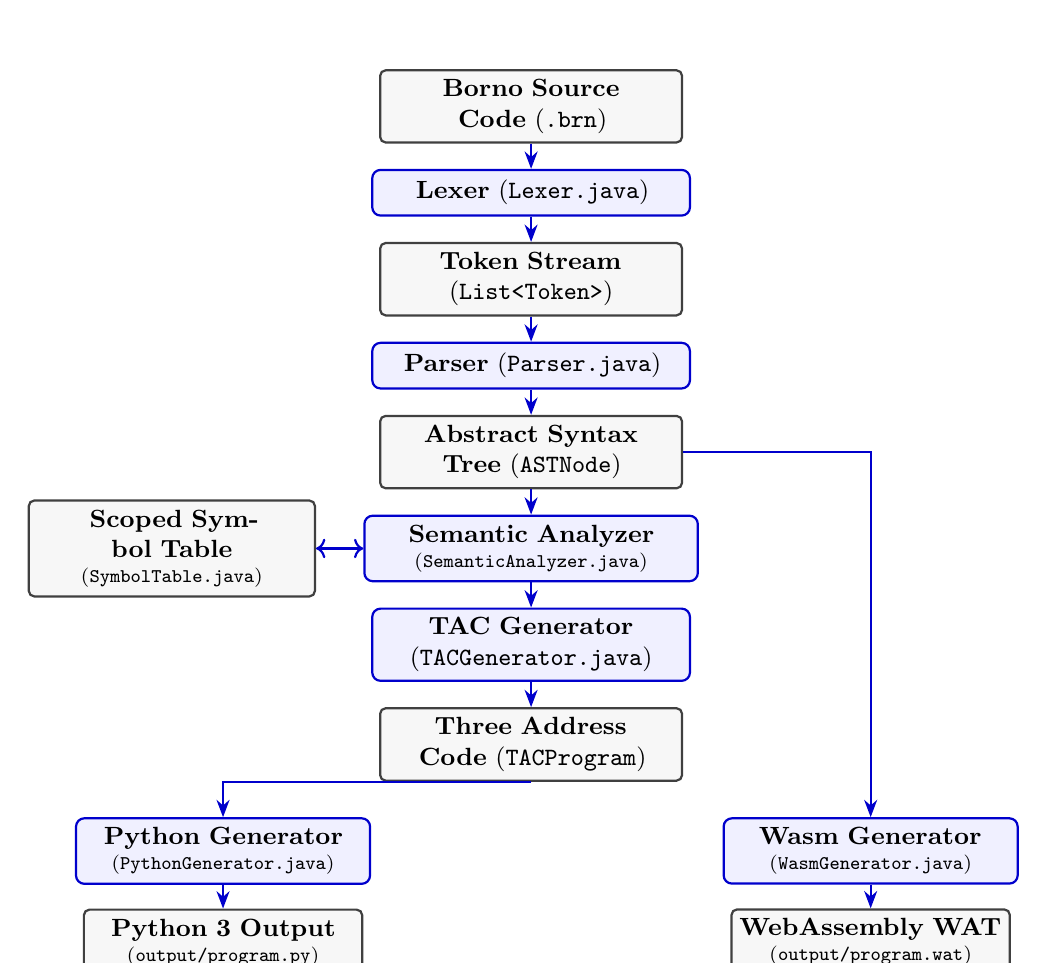
\begin{tikzpicture}[
    node distance=0.32cm and 0.8cm,
    every node/.style={font=\small},
    phase/.style={rectangle, draw=blue!80!black, fill=blue!6, thick, text width=3.8cm, align=center, minimum height=0.58cm, rounded corners=3pt},
    artifact/.style={rectangle, draw=black!75, fill=gray!6, thick, text width=3.6cm, align=center, minimum height=0.55cm, rounded corners=2pt},
    arrow/.style={-{Stealth[length=2.2mm]}, thick, draw=blue!80!black}
]
    % Central Pipeline Nodes
    \node[artifact] (source) {\textbf{Borno Source Code} (\texttt{.brn})};
    \node[phase, below=of source] (lexer) {\textbf{Lexer} (\texttt{Lexer.java})};
    \node[artifact, below=of lexer] (tokens) {\textbf{Token Stream} (\texttt{List<Token>})};
    \node[phase, below=of tokens] (parser) {\textbf{Parser} (\texttt{Parser.java})};
    \node[artifact, below=of parser] (ast) {\textbf{Abstract Syntax Tree} (\texttt{ASTNode})};
    \node[phase, below=of ast, text width=4.0cm] (semantic) {\textbf{Semantic Analyzer}\\[-2pt]{\scriptsize(\texttt{SemanticAnalyzer.java})}};
    
    % Scoped Symbol Table placed to the LEFT of Semantic Analyzer (no arrow crossing!)
    \node[artifact, left=0.6cm of semantic, text width=3.4cm] (symtab) {\textbf{Scoped Symbol Table}\\[-2pt]{\scriptsize(\texttt{SymbolTable.java})}};
    
    \node[phase, below=of semantic] (tacgen) {\textbf{TAC Generator} (\texttt{TACGenerator.java})};
    \node[artifact, below=of tacgen] (tac) {\textbf{Three Address Code} (\texttt{TACProgram})};
    
    % Target Generators placed side-by-side below
    \node[phase, below left=0.45cm and 0.1cm of tac, text width=3.5cm] (pygen) {\textbf{Python Generator}\\[-2pt]{\scriptsize(\texttt{PythonGenerator.java})}};
    \node[phase, below right=0.45cm and 0.5cm of tac, text width=3.5cm] (wasmgen) {\textbf{Wasm Generator}\\[-2pt]{\scriptsize(\texttt{WasmGenerator.java})}};
    
    \node[artifact, below=0.3cm of pygen, text width=3.3cm] (pyout) {\textbf{Python 3 Output}\\[-2pt]{\scriptsize(\texttt{output/program.py})}};
    \node[artifact, below=0.3cm of wasmgen, text width=3.3cm] (watout) {\textbf{WebAssembly WAT}\\[-2pt]{\scriptsize(\texttt{output/program.wat})}};
    
    % Flow Arrows
    \draw[arrow] (source) -- (lexer);
    \draw[arrow] (lexer) -- (tokens);
    \draw[arrow] (tokens) -- (parser);
    \draw[arrow] (parser) -- (ast);
    \draw[arrow] (ast) -- (semantic);
    \draw[arrow, <->] (semantic) -- (symtab);
    \draw[arrow] (semantic) -- (tacgen);
    \draw[arrow] (tacgen) -- (tac);
    \draw[arrow] (tac.south) -| (pygen.north);
    
    % Direct uncrossed route from AST to WasmGenerator along the clear right side
    \draw[arrow] (ast.east) -| (wasmgen.north);
    
    \draw[arrow] (pygen) -- (pyout);
    \draw[arrow] (wasmgen) -- (watout);
\end{tikzpicture}
\caption{Overall Architecture and Data Flow of BornoCompiler}
\label{fig:compiler_arch}
\end{figure}

% ─── Chapter 5: Phase-by-Phase Implementation ────────────────────────────────
\chapter{Phase-by-Phase Implementation}

\section{Phase 1: Lexical Analysis}
\begin{itemize}
    \item \textbf{Purpose}: Converts raw Bangla source text into a stream of tokens while filtering whitespace and comments.
    \item \textbf{Input}: Source code string.
    \item \textbf{Processing}: Character-by-character scanning with position tracking (\texttt{line}, \texttt{col}). It enforces native Bangla Unicode validation and maps keyword strings to \texttt{TokenType} enums.
    \item \textbf{Output}: A \texttt{List<Token>} terminated by \texttt{TokenType.EOF}.
    \item \textbf{Important Classes}: \texttt{Lexer}, \texttt{Token}, \texttt{TokenType}, \texttt{NumberHelper}.
    \item \textbf{Important Methods}: \texttt{nextToken()}, \texttt{tokenize()}, \texttt{readNumber()}, \texttt{readString()}, and \texttt{readIdentifierOrKeyword()}.
\end{itemize}

\section{Phase 2: Syntax Analysis (Parser)}
\begin{itemize}
    \item \textbf{Purpose}: Validates token sequences against the Borno grammar and constructs an Abstract Syntax Tree.
    \item \textbf{Input}: \texttt{List<Token>} produced by the Lexer.
    \item \textbf{Processing}: LL(1) recursive-descent parsing with precedence climbing. Uses panic-mode error recovery (\texttt{synchronize()}) to avoid cascading failures.
    \item \textbf{Output}: A \texttt{ProgramNode} representing the program root.
    \item \textbf{Important Classes}: \texttt{Parser}, \texttt{ASTNode}, \texttt{ASTPrinter}.
    \item \textbf{Important Methods}: \texttt{parseProgram()}, \texttt{parseStatement()}, \texttt{parseDeclare()}, \texttt{parseIf()}, \texttt{parseWhile()}, \texttt{parseFor()}, \texttt{consume()}, and \texttt{synchronize()}.
\end{itemize}

\section{Phase 3: Semantic Analysis}
\begin{itemize}
    \item \textbf{Purpose}: Validates language semantics, ensures variables are declared before use, and checks type compatibility.
    \item \textbf{Input}: \texttt{ProgramNode} AST.
    \item \textbf{Processing}: Traverses the AST while managing scoped symbol tables. Evaluates constant expressions at compile time to detect division by zero.
    \item \textbf{Output}: Semantic validation logs, populated symbol table, or semantic error exceptions.
    \item \textbf{Important Classes}: \texttt{SemanticAnalyzer}, \texttt{SymbolTable}, \texttt{Type}.
    \item \textbf{Important Methods}: \texttt{analyze()}, \texttt{analyzeAssignment()}, \texttt{analyzeIf()}, \texttt{analyzeWhile()}, \texttt{analyzeFor()}, and \texttt{evaluateConstant()}.
\end{itemize}

\section{Phase 4: Intermediate Code Generation (TAC)}
\begin{itemize}
    \item \textbf{Purpose}: Flattens the hierarchical AST into a linear stream of Three Address Code instructions.
    \item \textbf{Input}: Validated \texttt{ProgramNode} AST.
    \item \textbf{Processing}: Generates sequential temporary variables (\texttt{t1}, \texttt{t2}, \dots) and control-flow labels (\texttt{L1}, \texttt{L2}, \dots).
    \item \textbf{Output}: A \texttt{TACProgram} containing \texttt{TACInstruction} objects.
    \item \textbf{Important Classes}: \texttt{TACGenerator}, \texttt{TACProgram}, \texttt{TACInstruction}.
    \item \textbf{Important Methods}: \texttt{generate()}, \texttt{generateStatement()}, \texttt{newTemp()}, \texttt{newLabel()}, and \texttt{writeToFile()}.
\end{itemize}

\section{Phase 5: Target Code Generation}
\begin{itemize}
    \item \textbf{Purpose}: Emits runnable Python 3 and WebAssembly Text Format source files.
    \item \textbf{Input}: \texttt{TACProgram} (for Python) and \texttt{ProgramNode} AST (for WebAssembly).
    \item \textbf{Processing}: 
    \begin{itemize}
        \item \textit{Python}: Pattern-matches TAC jumps to reconstruct indented \texttt{if} and \texttt{while} structures; translates operators and converts Bangla digits.
        \item \textit{WebAssembly}: Allocates local variables, writes strings into linear memory data segments, and emits stack bytecode instructions.
    \end{itemize}
    \item \textbf{Output}: \texttt{output/program.py}, \texttt{output/program.wat}, and\\ compiled \texttt{output/program.wasm}.
    \item \textbf{Important Classes}: \texttt{PythonGenerator}, \texttt{WasmGenerator}.
    \item \textbf{Important Methods}: \texttt{PythonGenerator.generate()}, \texttt{WasmGenerator.generate()}, and \texttt{compileWatToWasm()}.
\end{itemize}

% ─── Chapter 6: UML Class Diagrams ───────────────────────────────────────────
\chapter{UML Class Diagrams}

This chapter details the object-oriented structure of BornoCompiler. The system architecture is organized into modular subsystems covering lexical scanning, syntax tree hierarchies, scoped semantic environments, three-address intermediate code representations, multi-target code synthesis, and the interactive compiler driver.

The design adheres to classical compiler engineering principles, isolating phase responsibilities while establishing clear data contracts between pipeline stages. Each subsystem is documented with its primary classes, fields, visibility qualifiers, and method contracts.

The subsequent sections dedicate a comprehensive page to each compiler subsystem, providing detailed structural descriptions alongside reserved spaces for visual UML class diagrams:
\begin{itemize}
    \item \textbf{Section 6.1}: \textit{Lexer and Token Module} (Figure \ref{fig:uml_lexer}) --- Token classification, coordinate tracking, and Bangla numeric conversion.
    \item \textbf{Section 6.2}: \textit{Parser and AST Hierarchy} (Figure \ref{fig:uml_parser_ast}) --- Composite AST nodes, statements, expressions, and recursive descent.
    \item \textbf{Section 6.3}: \textit{Semantic Analysis Module} (Figure \ref{fig:uml_semantic}) --- Scoped symbol resolution, static types, and compile-time evaluation.
    \item \textbf{Section 6.4}: \textit{Three Address Code Module} (Figure \ref{fig:uml_tac}) --- Linear intermediate representation, temporary registers, and jump labels.
    \item \textbf{Section 6.5}: \textit{Target Code Generation Module} (Figure \ref{fig:uml_codegen}) --- Python 3 structured generation and WebAssembly Text Format emission.
    \item \textbf{Section 6.6}: \textit{Driver and Pipeline Architecture} (Figure \ref{fig:uml_pipeline}) --- Central CLI runner, runtime execution harness, and test runner.
\end{itemize}

Interactive visual diagrams and their source representations can be accessed in \path{diagrams/view_uml.html}.

\clearpage
\section{Lexer and Token Module UML Class Diagram}
The lexical analysis subsystem converts the raw Bangla source string into a stream of strongly typed tokens with line and column coordinates. It comprises four primary components: \textbf{\texttt{TokenType}} (enumerates 24 token kinds including language keywords, literals, arithmetic/relational operators, and delimiters), \textbf{\texttt{Token}} (encapsulates classification type, string value, and 1-based source coordinates), \textbf{\texttt{NumberHelper}} (static utility routines for bidirectional conversion between Bangla and ASCII digits and numeric validation), and \textbf{\texttt{Lexer}} (the scanning engine managing coordinate pointers, Unicode character classification, and lexical error reporting).

\umlspacesection{fig:uml_lexer}{Lexer and Token Module UML Class Diagram}{diagrams/fig_6_1_lexer.png}{height=15.5cm, keepaspectratio}

\clearpage
\section{Parser and AST Hierarchy UML Class Diagram}
The syntactic analysis subsystem parses the token stream into a typed Abstract Syntax Tree (AST) using an LL(1) recursive-descent strategy. The AST hierarchy is rooted at the abstract \textbf{\texttt{ASTNode}} base class, extended by statement nodes (\texttt{ProgramNode}, \texttt{BlockNode}, \texttt{AssignmentNode}, \texttt{IfNode}, \texttt{WhileNode}, \texttt{ForNode}, \texttt{PrintNode}) and expression nodes (\texttt{BinaryExpressionNode}, \texttt{UnaryExpressionNode}, \texttt{VariableNode}, \texttt{LiteralNode}). The \textbf{\texttt{Parser}} coordinates grammar productions, operator precedence, and panic-mode synchronization, while \textbf{\texttt{ASTPrinter}} provides hierarchical tree visualization.

\umlspacesection{fig:uml_parser_ast}{Parser and AST Hierarchy UML Class Diagram}{diagrams/fig_6_2_parser.png}{width=1.06\textwidth, height=12.0cm, keepaspectratio}

\clearpage
\section{Semantic Analysis Module UML Class Diagram}
The semantic analysis subsystem verifies static type safety, identifier declaration scopes, and constant expressions. Key components include \textbf{\texttt{Type}} (enumerates static types \texttt{NUMBER}, \texttt{STRING}, \texttt{BOOLEAN}, and \texttt{UNKNOWN} with native Bangla diagnostic strings), \textbf{\texttt{SymbolTable}} (hierarchical scoped environment storing symbol types, initialization states, constant values, and parent scope pointers), and \textbf{\texttt{SemanticAnalyzer}} (walks the AST to perform scoped validation, type checking, and compile-time division-by-zero detection).

\umlspacesection{fig:uml_semantic}{Semantic Analysis Module UML Class Diagram}{diagrams/fig_6_3_semantic.png}{height=16.2cm, keepaspectratio}

\clearpage
\section{Three Address Code (TAC) Module UML Class Diagram}
The intermediate representation subsystem linearizes nested expressions and hierarchical control flow into three-address quadruples. The module comprises \textbf{\texttt{OpType}} (defines the eight instruction variants including binary, unary, assignment, branching, and labels), \textbf{\texttt{TACInstruction}} (encapsulates operator, operands, result, and static factory constructors), \textbf{\texttt{TACProgram}} (container managing the sequential instruction sequence and formatting printable output), and \textbf{\texttt{TACGenerator}} (lowers AST constructs into temporaries \texttt{t1}, \texttt{t2} and branch labels \texttt{L1}, \texttt{L2}).

\umlspacesection{fig:uml_tac}{Three Address Code (TAC) Module UML Class Diagram}{diagrams/fig_6_4_tac.png}{height=15.5cm, keepaspectratio}

\clearpage
\section{Target Code Generation Module UML Class Diagram}
The code generation subsystem translates intermediate representations into runnable target formats. It comprises \textbf{\texttt{PythonGenerator}} (converts TAC instruction sequences into clean, indented Python 3 source code by reconstructing structured \texttt{if}, \texttt{else}, and \texttt{while} blocks and converting Bangla numerals to ASCII digits) and \textbf{\texttt{WasmGenerator}} (traverses the AST to emit stack-oriented WebAssembly Text Format \texttt{.wat}, manages local variable indices, allocates linear memory for string constants, and invokes \texttt{wat2wasm} to generate binary \texttt{.wasm} packages).

\umlspacesection{fig:uml_codegen}{Target Code Generation Module UML Class Diagram}{diagrams/fig_6_5_codegen.png}{width=1.04\textwidth, height=12.5cm, keepaspectratio}

\clearpage
\section{Driver and Pipeline Architecture UML Class Diagram}
The compiler driver and test pipeline coordinate all compilation stages and provide automated regression testing. The module features \textbf{\texttt{Main}} (the primary interactive command-line interface managing stage-by-stage execution from lexing to Python and WebAssembly execution, custom source input handling, and test-suite invocation) and \textbf{\texttt{TestRunner}} (the standalone automated test harness that executes the 28 comprehensive test cases and validates compiler output across all subsystems).

\umlspacesection{fig:uml_pipeline}{Compiler Pipeline and Driver UML Class Diagram}{diagrams/fig_6_6_pipeline.png}{width=1.04\textwidth, height=13.0cm, keepaspectratio}

% ─── Chapter 7: TAC Design ───────────────────────────────────────────────────
\chapter{Intermediate Representation (Three Address Code Design)}

\section{Principles of Three Address Code}
Three Address Code (TAC) is an intermediate representation where instructions have at most one operator and at most three addresses:
\[
\text{Result} = \text{Operand}_1 \quad \text{Operator} \quad \text{Operand}_2
\]

\section{Why TAC is Used in BornoCompiler}
\begin{enumerate}
    \item \textbf{Decoupling}: Separates language parsing from target code emission.
    \item \textbf{Control-Flow Normalization}: High-level loops and branches are simplified into conditional and unconditional jumps.
    \item \textbf{Target Extensibility}: Adding new target architectures requires only reading the linear TAC instruction stream.
\end{enumerate}

\section{TACInstruction Representation}
Implemented in \texttt{TACInstruction.java}, each instruction stores:
\begin{itemize}
    \item \texttt{opType}: The instruction category from \texttt{OpType}.
    \item \texttt{result}: Target variable, allocated temporary, or jump label.
    \item \texttt{arg1}: First source operand.
    \item \texttt{op}: Operator string.
    \item \texttt{arg2}: Second source operand (if applicable).
\end{itemize}

\section{TACProgram Container}
\texttt{TACProgram.java} stores instructions and provides two serialization outputs:
\begin{enumerate}
    \item \textbf{Annotated Bangla Output}: Used in compiler educational logs:
\begin{lstlisting}
১. [Copy] বয়স = ২০
২. [BinOp] t1 = বয়স >= ১৮
৩. [IfFalseGoto] শর্ত t1 মিথ্যা হলে L1-এ যাও
\end{lstlisting}
    \item \textbf{Raw TAC Output}: Formatted as conventional compiler IR:
\begin{lstlisting}
    বয়স = ২০
    t1 = বয়স >= ১৮
    ifFalse t1 goto L1
\end{lstlisting}
\end{enumerate}

\section{TACGenerator Lowering Logic}
\texttt{TACGenerator.java} lowers AST nodes as follows:
\begin{itemize}
    \item \textbf{Assignment}: Evaluates the expression and emits \texttt{ASSIGN\_COPY}.
    \item \textbf{Print}: Evaluates the expression and emits \texttt{PRINT}.
    \item \textbf{If-Else}: Evaluates the condition, emits \texttt{ifFalseGoto} targeting the else-label, lowers the then-block, emits \texttt{goto} targeting the end-label, and places labels appropriately.
    \item \textbf{While Loop}: Emits a start label, evaluates the condition, emits an \texttt{ifFalseGoto} to the exit label, lowers body statements, emits an unconditional jump back to the start label, and places the exit label.
\end{itemize}

\section{Supported TAC Operations}
\begin{table}[htbp]
\centering
\small
\renewcommand{\arraystretch}{1.25}
\begin{tabular}{|l|l|l|}
\hline
\textbf{OpType Enum} & \textbf{Raw Syntax} & \textbf{Bangla Annotated Format} \\
\hline
\texttt{ASSIGN\_BINARY} & \texttt{t1 = a + b} & \texttt{[BinOp] t1 = a + b} \\
\hline
\texttt{ASSIGN\_UNARY} & \texttt{t1 = -a} & \texttt{[Unary] t1 = -a} \\
\hline
\texttt{ASSIGN\_COPY} & \texttt{x = t1} & \texttt{[Copy] x = t1} \\
\hline
\texttt{PRINT} & \texttt{print x} & \texttt{[Print] দেখাও(x)} \\
\hline
\texttt{IF\_FALSE\_GOTO} & \texttt{ifFalse t1 goto L1} & \texttt{[IfFalseGoto] শর্ত t1 মিথ্যা হলে L1-এ যাও} \\
\hline
\texttt{IF\_GOTO} & \texttt{if t1 goto L1} & \texttt{[IfGoto] শর্ত t1 সত্য হলে L1-এ যাও} \\
\hline
\texttt{GOTO} & \texttt{goto L2} & \texttt{[Goto] যাও L2} \\
\hline
\texttt{LABEL} & \texttt{L1:} & \texttt{[Label] L1:} \\
\hline
\end{tabular}
\caption{Supported TAC Operations in BornoCompiler}
\label{tab:tac_ops}
\end{table}

\section{Temporary Variable Management}
Temporaries are allocated sequentially via \texttt{newTemp()} as \texttt{t1}, \texttt{t2}, \texttt{t3}, \dots to hold subexpression results during arithmetic evaluation.

\section{Labels and Control Flow Flattening}
Symbolic labels are generated via \texttt{newLabel()} as \texttt{L1}, \texttt{L2}, \texttt{L3}, \dots to mark branch targets and loop boundaries.

\section{Detailed TAC Translation Example}
For the input:
\begin{lstlisting}
ধরি সংখ্যা ক = ১০ + ২০ * ৫;
\end{lstlisting}
The multiplication subexpression is evaluated first due to precedence climbing, yielding:
\begin{lstlisting}
১. [BinOp] t1 = ২০ * ৫
২. [BinOp] t2 = ১০ + t1
৩. [Copy]  ক = t2
\end{lstlisting}

% ─── Chapter 8: Target Code Generation ───────────────────────────────────────
\chapter{Target Code Generation}

\section{Python Code Generator}
\texttt{PythonGenerator.java} translates TAC instructions into executable Python 3. It detects branch and jump patterns to generate properly indented blocks, converts Bangla numbers using \texttt{NumberHelper.toAsciiDigits()}, and configures UTF-8 encoding on standard output.

\section{WebAssembly (WAT) Code Generator}
\texttt{WasmGenerator.java} translates the AST into WebAssembly Text Format (\texttt{.wat}). Variables become local \texttt{i32} registers, strings are placed in linear memory data segments, and expressions are emitted as stack operations.

\section{TAC-to-Python Translation Workflow}
\begin{enumerate}
    \item Pattern-matches TAC jump instructions to identify block structures.
    \item Recursively generates indented blocks for \texttt{if}, \texttt{else}, and \texttt{while} constructs.
    \item Translates operators (\texttt{এবং} $\rightarrow$ \texttt{and}, \texttt{অথবা} $\rightarrow$ \texttt{or}, \texttt{না} $\rightarrow$ \texttt{not}).
    \item Writes formatted code to \texttt{output/program.py}.
\end{enumerate}

\section{AST-to-WAT Translation Workflow}
\begin{enumerate}
    \item Scans the AST to identify all variables and string literals.
    \item Emits module headers, runtime imports (\texttt{\$print\_i32}, \texttt{\$print\_str}), and memory exports.
    \item Emits data segments for string constants with null terminators.
    \item Emits function \texttt{\$main} containing local variable declarations and statement instructions.
    \item Invokes \texttt{wat2wasm} if present to compile \texttt{output/program.wasm}.
\end{enumerate}

\section{Example Target Code}
For the program:
\begin{lstlisting}
ধরি সংখ্যা বয়স = ২০;
যদি (বয়স >= ১৮) {
    ধরি সংখ্যা অবস্থা = ১;
} নাহলে {
    ধরি সংখ্যা অবস্থা = ০;
}
\end{lstlisting}

\noindent\textbf{Generated Python 3 (\texttt{output/program.py})}:
\begin{lstlisting}[language=Python]
# -*- coding: utf-8 -*-
import sys
if hasattr(sys.stdout, 'reconfigure'):
    sys.stdout.reconfigure(encoding='utf-8')

বয়স = 20
t1 = বয়স >= 18
if t1:
    অবস্থা = 1
else:
    অবস্থা = 0
\end{lstlisting}

\noindent\textbf{Generated WebAssembly Text Format (\texttt{output/program.wat})}:
\begin{lstlisting}
(module
  (import "env" "print_i32" (func $print_i32 (param i32)))
  (import "env" "print_str" (func $print_str (param i32 i32)))
  (memory (export "memory") 1)

  (func $main (export "main")
    (local $var_0 i32)  ;; বয়স
    (local $var_1 i32)  ;; অবস্থা

    i32.const 20
    local.set $var_0
    local.get $var_0
    i32.const 18
    i32.ge_s
    if
      i32.const 1
      local.set $var_1
    else
      i32.const 0
      local.set $var_1
    end
  )
)
\end{lstlisting}

% ─── Chapter 9: Language Grammar ─────────────────────────────────────────────
\chapter{Language Grammar}

\section{Grammar Introduction}
The formal grammar of Borno is derived directly from \texttt{Parser.java}. It is an unambiguous, context-free grammar designed for deterministic LL(1) parsing.

\section{Complete BNF Grammar}
\begin{lstlisting}[basicstyle=\ttfamily\footnotesize]
<program> ::= <statement_list> EOF

<statement_list> ::= <statement> <statement_list>
                   | epsilon

<statement> ::= <declare_stmt>
              | <reassign_stmt>
              | <print_stmt>
              | <if_stmt>
              | <while_stmt>
              | <for_stmt>

<declare_stmt> ::= 'ধরি' <type_specifier> IDENTIFIER '=' <expression> ';'
                 | <type_specifier> IDENTIFIER '=' <expression> ';'

<type_specifier> ::= 'সংখ্যা'
                   | 'বাক্য'
                   | 'লেখা'

<reassign_stmt> ::= IDENTIFIER '=' <expression> ';'

<print_stmt> ::= 'দেখাও' '(' <expression> ')' ';'

<if_stmt> ::= 'যদি' '(' <expression> ')' <block> <else_opt>

<else_opt> ::= 'নাহলে' <block>
             | epsilon

<while_stmt> ::= 'যতক্ষণ' '(' <expression> ')' <block>

<for_stmt> ::= <for_keyword> '(' <for_init> <for_cond> <for_update> ')' <block>

<for_keyword> ::= 'ফর' | 'for' | 'জন্য' | 'প্রতি' | 'প্রতিটি'

<for_init> ::= <declare_stmt>
             | <reassign_stmt>
             | <expression> ';'
             | ';'

<for_cond> ::= <expression> ';'
             | ';'

<for_update> ::= IDENTIFIER '=' <expression>
               | <expression>
               | epsilon

<block> ::= '{' <statement_list> '}'

<expression> ::= <comparison>

<comparison> ::= <addition> ( <rel_op> <addition> )*

<rel_op> ::= '==' | '!=' | '<' | '>' | '<=' | '>='

<addition> ::= <multiplication> ( <add_op> <multiplication> )*

<add_op> ::= '+' | '-'

<multiplication> ::= <unary> ( <mul_op> <unary> )*

<mul_op> ::= '*' | '/' | '%'

<unary> ::= '-' <unary>
          | '+' <unary>
          | '!' <unary>
          | 'না' <unary>
          | <primary>

<primary> ::= NUMBER
            | STRING
            | IDENTIFIER
            | '(' <expression> ')'
\end{lstlisting}

\section{Explanation of Major Grammar Rules}
\begin{itemize}
    \item \textbf{Precedence Hierarchy}: Stratified productions enforce standard algebraic order of operations (\texttt{comparison} $\rightarrow$ \texttt{addition} $\rightarrow$ \texttt{multiplication} $\rightarrow$ \texttt{unary} $\rightarrow$ \texttt{primary}).
    \item \textbf{Left Associativity}: Binary operators are parsed iteratively in \texttt{Parser.java} using loops, establishing left-associative tree construction.
    \item \textbf{Right Associativity}: Unary operators are parsed via direct recursion, establishing right-associative binding.
\end{itemize}

% ─── Chapter 10: End-to-End Compilation ──────────────────────────────────────
\chapter{Example End-to-End Compilation Walkthrough}

This chapter traces the complete end-to-end compilation lifecycle of a representative Borno source program. The walkthrough demonstrates how each phase of the BornoCompiler pipeline transforms the program—progressing sequentially from raw source text to lexical tokens, an Abstract Syntax Tree (AST), scoped symbol resolution, linear Three Address Code (TAC), and final target code generation in Python 3 and WebAssembly.

\section*{Sample Source Program}
The example program declares two integer variables (\texttt{ক} and \texttt{খ}), computes an arithmetic expression with nested operator precedence (\texttt{৫ * ২} before addition with \texttt{ক}), and prints the resulting value using the native \texttt{দেখাও} statement:

\begin{tcolorbox}[colback=codegray,colframe=black!20,arc=0mm,boxrule=0.5pt,left=10pt,right=10pt,top=6pt,bottom=6pt]
\ttfamily\small
ধরি সংখ্যা ক = ১০;\\
ধরি সংখ্যা খ = ক + ৫ * ২;\\
দেখাও(খ);
\end{tcolorbox}

The following sections illustrate the concrete intermediate representations and outputs synthesized at each compiler milestone.

\section{Tokens Generated by Lexer}
\begin{tcolorbox}[colback=codegray,colframe=black!20,arc=0mm,boxrule=0.5pt,left=10pt,right=10pt,top=4pt,bottom=4pt]
\ttfamily\small
\begin{tabular}{@{}l@{\quad:\quad}l@{\qquad}l@{}}
DHORI       & 'ধরি'      & (লাইন ১) \\
SONGKHA     & 'সংখ্যা'    & (লাইন ১) \\
IDENTIFIER  & 'ক'        & (লাইন ১) \\
ASSIGN      & '='        & (লাইন ১) \\
NUMBER      & '১০'       & (লাইন ১) \\
SEMICOLON   & ';'        & (লাইন ১) \\
DHORI       & 'ধরি'      & (লাইন ২) \\
SONGKHA     & 'সংখ্যা'    & (লাইন ২) \\
IDENTIFIER  & 'খ'        & (লাইন ২) \\
ASSIGN      & '='        & (লাইন ২) \\
IDENTIFIER  & 'ক'        & (লাইন ২) \\
PLUS        & '+'        & (লাইন ২) \\
NUMBER      & '৫'        & (লাইন ২) \\
MULTIPLY    & '*'        & (লাইন ২) \\
NUMBER      & '২'        & (লাইন ২) \\
SEMICOLON   & ';'        & (লাইন ২) \\
DEKHAO      & 'দেখাও'    & (লাইন ৩) \\
LEFT\_PAREN & '('        & (লাইন ৩) \\
IDENTIFIER  & 'খ'        & (লাইন ৩) \\
RIGHT\_PAREN& ')'        & (লাইন ৩) \\
SEMICOLON   & ';'        & (লাইন ৩) \\
EOF         & ''         & (লাইন ৪)
\end{tabular}
\end{tcolorbox}

\section{Abstract Syntax Tree (AST)}
\begin{tcolorbox}[colback=codegray,colframe=black!20,arc=0mm,boxrule=0.5pt,left=10pt,right=10pt,top=4pt,bottom=4pt]
\ttfamily\small
PROGRAM\\
|\\
+-- DECLARATION\\
|~~~~+-- TYPE~~: সংখ্যা\\
|~~~~+-- NAME~~: ক\\
|~~~~`-- VALUE~: ১০\\
|\\
+-- DECLARATION\\
|~~~~+-- TYPE~~: সংখ্যা\\
|~~~~+-- NAME~~: খ\\
|~~~~`-- VALUE~: (ক + (৫ * ২))\\
|\\
`-- PRINT\\
~~~~~`-- EXPR~~: খ
\end{tcolorbox}

\section{Semantic Analysis Output}
\begin{tcolorbox}[colback=codegray,colframe=black!20,arc=0mm,boxrule=0.5pt,left=10pt,right=10pt,top=4pt,bottom=4pt]
\ttfamily\small
Symbol Table:\\[2pt]
\begin{tabular}{|l|l|l|}
\hline
\textbf{Name} & \textbf{Type} & \textbf{Initialized} \\
\hline
ক & সংখ্যা & হ্যাঁ \\
খ & সংখ্যা & হ্যাঁ \\
\hline
\end{tabular}\\[8pt]
Semantic Check Logs:\\
{[}OK{]} ক -> সংখ্যা\\
{[}OK{]} খ -> সংখ্যা\\
{[}OK{]} PRINT statement valid
\end{tcolorbox}

\clearpage
\section{Three Address Code Output}
\begin{tcolorbox}[colback=codegray,colframe=black!20,arc=0mm,boxrule=0.5pt,left=10pt,right=10pt,top=3pt,bottom=3pt,before=\vspace{1pt},after=\vspace{3pt}]
\ttfamily\small
১. [Copy] ক = ১০\\
২. [BinOp] t1 = ৫ * ২\\
৩. [BinOp] t2 = ক + t1\\
৪. [Copy] খ = t2\\
৫. [Print] দেখাও(খ)
\end{tcolorbox}

\section{Target Code Outputs}

\noindent\textbf{Python 3 Output (\texttt{output/program.py})}:

\begin{tcolorbox}[colback=codegray,colframe=black!20,arc=0mm,boxrule=0.5pt,left=10pt,right=10pt,top=3pt,bottom=3pt,before=\vspace{1pt},after=\vspace{3pt}]
\ttfamily\small
\# -*- coding: utf-8 -*-\\
import sys\\
if hasattr(sys.stdout, 'reconfigure'):\\
\mbox{}~~~~sys.stdout.reconfigure(encoding='utf-8')\\
ক = 10\\
t1 = 5 * 2\\
t2 = ক + t1\\
খ = t2\\
print(খ)
\end{tcolorbox}

\par\vspace{2pt}
\noindent\textbf{WebAssembly Output (\texttt{output/program.wat})}:

\begin{lstlisting}[basicstyle=\ttfamily\footnotesize, aboveskip=2pt, belowskip=2pt]
(module
  (import "env" "print_i32" (func $print_i32 (param i32)))
  (import "env" "print_str" (func $print_str (param i32 i32)))
  (memory (export "memory") 1)

  (func $main (export "main")
    (local $var_0 i32)  ;; ক
    (local $var_1 i32)  ;; খ
    i32.const 10
    local.set $var_0
    local.get $var_0
    i32.const 5
    i32.const 2
    i32.mul
    i32.add
    local.set $var_1
    local.get $var_1
    call $print_i32
  )
)
\end{lstlisting}

% ─── Chapter 11: Testing and Validation ──────────────────────────────────────
\chapter{Testing and Validation}

\section{Automated Test Suite (28 Test Cases)}
The compiler includes an automated test harness embedded directly in \texttt{Main.java}. Table~\ref{tab:test_suite} summarizes the test cases and their execution outcomes:

\renewcommand{\arraystretch}{1.25}
\noindent\begin{longtable}{|c|>{\raggedright\arraybackslash}p{2.8cm}|>{\raggedright\arraybackslash}p{3.8cm}|>{\raggedright\arraybackslash}p{3.8cm}|c|}
\hline
\textbf{ID} & \textbf{Test Name} & \textbf{Input Snippet} & \textbf{Expected Outcome} & \textbf{Result} \\
\hline
\endfirsthead
\hline
\textbf{ID} & \textbf{Test Name} & \textbf{Input Snippet} & \textbf{Expected Outcome} & \textbf{Result} \\
\hline
\endhead
\hline
\endfoot
\hline
\caption{Automated Test Suite Results (Main.java)}
\label{tab:test_suite}
\endlastfoot
1 & Bangla Digits Accepted & \texttt{ধরি সংখ্যা বয়স = ২০;} & Success & PASS \\
\hline
2 & English Digits Rejected & \texttt{ধরি সংখ্যা বয়স = 20;} & Lexical Error & PASS \\
\hline
3 & Bangla Identifier Accepted & \texttt{ধরি সংখ্যা বয়স = ২০;} & Success & PASS \\
\hline
4 & English Identifier Rejected & \texttt{ধরি সংখ্যা age = ২০;} & Lexical Error & PASS \\
\hline
5 & Mixed Identifier Rejected & \texttt{ধরি সংখ্যা বয়স123 = ২০;} & Lexical Error & PASS \\
\hline
6 & English Keyword Rejected & \texttt{if (বয়স >= ১৮) \{ \dots \}} & Lexical Error & PASS \\
\hline
7 & Mixed Keyword Rejected & \texttt{dhori সংখ্যা বয়স = ২০;} & Lexical Error & PASS \\
\hline
8 & Valid Multi-statement Demo & Complete demo program & Success & PASS \\
\hline
9 & Type Mismatch & \texttt{ধরি সংখ্যা বয়স = "মাহদি";} & Semantic Error & PASS \\
\hline
10 & Division by Zero & \texttt{ধরি সংখ্যা ফলাফল = ১০ / ০;} & Semantic Error & PASS \\
\hline
11 & Undeclared Variable in Print & \texttt{দেখাও(নাম);} & Semantic Error & PASS \\
\hline
12 & Undeclared Variable in Expr & \texttt{ধরি সংখ্যা ফলাফল = বয়স + ১০;} & Semantic Error & PASS \\
\hline
13 & Duplicate Declaration & \texttt{ধরি সংখ্যা বয়স = ২০; \dots} & Semantic Error & PASS \\
\hline
14 & Non-Boolean IF Condition & \texttt{যদি (বয়স) \{ \dots \}} & Semantic Error & PASS \\
\hline
15 & Missing Semicolon & \texttt{ধরি সংখ্যা বয়স = ২০} & Syntax Error & PASS \\
\hline
16 & Invalid Character & \texttt{ধরি সংখ্যা \$বয়স = ২০;} & Lexical Error & PASS \\
\hline
17 & Unclosed String & \texttt{ধরি বাক্য বার্তা = "অসমাপ্ত;} & Lexical Error & PASS \\
\hline
18 & Valid Number \& String & Variable declarations & Success & PASS \\
\hline
19 & Operator Precedence & \texttt{১০ + ২০ * ৩ - ৫} & Success & PASS \\
\hline
20 & String Print Statement & String output via \texttt{দেখাও} & Success & PASS \\
\hline
21 & Nested IF and Scoping & Block-scoped variables & Success & PASS \\
\hline
22 & Full Demo Program & Conditional branching demo & Success & PASS \\
\hline
23 & Valid Unary Expression & \texttt{ধরি সংখ্যা ক = -৫;} & Success & PASS \\
\hline
24 & Valid While Loop & \texttt{যতক্ষণ (ক < ৫) \{ \dots \}} & Success & PASS \\
\hline
25 & Valid For Loop & \texttt{for (ক=০; ক<৫; ক=ক+১)} & Success & PASS \\
\hline
26 & Nested Loop in Conditional & While inside if condition & Success & PASS \\
\hline
27 & Non-Boolean While Condition & \texttt{যতক্ষণ (ক) \{ \dots \}} & Semantic Error & PASS \\
\hline
28 & Intentional Failure Test & Valid division evaluated against expected error & Harness verification & EXP. FAIL \\
\hline
\end{longtable}

\section{Dedicated Regression Runner}
\texttt{TestRunner.java} provides regression verification across 12 targeted scenarios focusing on loop latches, unary operators, and nested scope isolation.

% ─── Chapter 12: Limitations ─────────────────────────────────────────────────
\chapter{Limitations}

To maintain technical accuracy, the current limitations of the implementation are documented below:
\begin{enumerate}
    \item \textbf{No User-Defined Functions}: Programs consist of a single top-level sequence of statements; functions and procedures are not yet supported.
    \item \textbf{No Array or Composite Structures}: Variables are limited to scalar types (\texttt{NUMBER}, \texttt{STRING}, \texttt{BOOLEAN}).
    \item \textbf{WebAssembly Integer Truncation}: In \texttt{WasmGenerator.java}, numeric values are cast to WebAssembly \texttt{i32} registers, truncating fractional values in WASM output (Python retains full double-precision support).
    \item \textbf{No Interactive Input Construct}: Terminal input statements (such as \texttt{ইনপুট()}) are not yet implemented.
\end{enumerate}

% ─── Chapter 13: Future Work ─────────────────────────────────────────────────
\chapter{Future Work}

Planned future enhancements include:
\begin{itemize}
    \item \textbf{Function Declarations}: Supporting user-defined functions with parameters and return values.
    \item \textbf{Arrays and Lists}: Adding support for indexed arrays (\texttt{তালিকা}).
    \item \textbf{Interactive Input}: Implementing an input construct for reading values from standard input.
    \item \textbf{Direct Bytecode Emission}: Compiling directly to JVM bytecode (\texttt{.class}) or native binaries via LLVM.
    \item \textbf{Bangla IDE}: Creating a graphical editor with syntax highlighting and inline diagnostic messages.
\end{itemize}

% ─── Chapter 14: Conclusion ──────────────────────────────────────────────────
\chapter{Conclusion}

BornoCompiler demonstrates a complete, working implementation of compiler construction principles applied to a native Bangla programming language. Built entirely from scratch in Java, the project implements an end-to-end six-phase pipeline: lexical scanning with coordinate tracking, recursive-descent LL(1) parsing with error recovery, Abstract Syntax Tree construction, scoped semantic analysis with compile-time constant evaluation, intermediate Three Address Code generation, and multi-target code emission for both Python 3 and WebAssembly.

Validated through automated test suites and sample programs, the compiler demonstrates that programming languages can be designed and implemented cleanly in non-Latin scripts, helping bridge educational gaps for Bangla-speaking computer science students.

% ─── References ──────────────────────────────────────────────────────────────
\begin{thebibliography}{9}

\bibitem{aho}
A. V. Aho, M. S. Lam, R. Sethi, and J. D. Ullman,
\textit{Compilers: Principles, Techniques, and Tools}, 2nd ed.
Addison-Wesley, 2006.

\bibitem{cooper}
K. D. Cooper and L. Torczon,
\textit{Engineering a Compiler}, 2nd ed.
Morgan Kaufmann, 2011.

\bibitem{nystrom}
R. Nystrom,
\textit{Crafting Interpreters}.
Genever Benning, 2021.

\bibitem{unicode}
The Unicode Consortium,
\textit{The Unicode Standard, Version 15.0: Bengali Script Block (Range: 0980--09FF)}.
Unicode, Inc., 2023.

\bibitem{wasm}
A. Haas et al.,
``Bringing the web up to speed with WebAssembly,''
in \textit{Proc. 38th ACM SIGPLAN Conf. on Programming Language Design and Implementation (PLDI)}, 2017, pp. 185--200.

\bibitem{python}
Python Software Foundation,
\textit{Python 3 Language Reference: Execution Model and Grammar}.
Available: \url{https://docs.python.org/3/reference/}, 2023.

\end{thebibliography}

% ─── Appendix ────────────────────────────────────────────────────────────────
\appendix
\chapter{Key Source Code Excerpts}

\section{Panic-Mode Synchronization in \texttt{Parser.java}}
\begin{lstlisting}[language=Java]
private void synchronize() {
    while (!check(TokenType.EOF)) {
        if (check(TokenType.SEMICOLON)) {
            advance();
            return;
        }
        if (check(TokenType.RIGHT_BRACE)) {
            return;
        }
        TokenType t = currentToken().getType();
        if (t == TokenType.DHORI || t == TokenType.SONGKHA || t == TokenType.BAKKA ||
            t == TokenType.JODI || t == TokenType.DEKHAO || t == TokenType.JOTOKKHON || t == TokenType.FOR) {
            return;
        }
        advance();
    }
}
\end{lstlisting}

\section[Static Division by Zero Detection in SemanticAnalyzer.java]{Static Division by Zero Detection in\\ \texttt{SemanticAnalyzer.java}}
\begin{lstlisting}[language=Java]
if (op.equals("/") || op.equals("%")) {
    Object rightVal = evaluateConstant(bin.getRight(), scope);
    if (rightVal instanceof Number && ((Number) rightVal).doubleValue() == 0.0) {
        String err = "[SEMANTIC ERROR]\nDivision by zero is not allowed.";
        errors.add(err);
        throw new RuntimeException(err);
    }
}
\end{lstlisting}

\chapter{Representative Borno Programs}

\section[Full Demo Program (valid\_full\_demo.brn)]{Full Demo Program (\texttt{valid\_full\_demo.brn})}
\begin{tcolorbox}[colback=codegray,colframe=black!20,arc=0mm,boxrule=0.5pt,left=10pt,right=10pt,top=4pt,bottom=4pt]
\ttfamily\small
ধরি সংখ্যা বয়স = ২০;\\
ধরি বাক্য নাম = "মাহদি";\\[6pt]
যদি (বয়স >= ১৮) \{\\
\mbox{}~~~~ধরি সংখ্যা অবস্থা = ১;\\
\mbox{}~~~~দেখাও("প্রাপ্তবয়স্ক");\\
\} নাহলে \{\\
\mbox{}~~~~ধরি সংখ্যা অবস্থা = ০;\\
\mbox{}~~~~দেখাও("অপ্রাপ্তবয়স্ক");\\
\}
\end{tcolorbox}

\section[While Loop with Nested Condition (TestRunner.java)]{While Loop with Nested Condition\\ (\texttt{TestRunner.java})}
\begin{tcolorbox}[colback=codegray,colframe=black!20,arc=0mm,boxrule=0.5pt,left=10pt,right=10pt,top=4pt,bottom=4pt]
\ttfamily\small
ধরি সংখ্যা ক = ০;\\[6pt]
যতক্ষণ (ক < ৫) \{\\
\mbox{}~~~~যদি (ক == ২) \{\\
\mbox{}~~~~~~~~দেখাও(ক);\\
\mbox{}~~~~\}\\
\mbox{}~~~~ক = ক + ১;\\
\}
\end{tcolorbox}

\end{document}
